\section{Vector Spaces}

  We begin with an axiomatic treatment of a \hyperref[alg-def:vector-space]{vector space}, which is one of the primary objects of study in linear algebra. Recall what a \hyperref[alg-def:field]{field} is from algebra. 

  Before we start, note that when students learn about vectors for the first time, they are presented with two interpretations of vectors. First, we think of a vector as an arrow pointing in space, encoding both a \textit{magnitude} and a \textit{direction}. This is more of the physicists interpretation and is useful in visualizing these vectors in low dimensions (notably, 2 and 3). 

  \begin{figure}[H]
    \centering
    \begin{subfigure}[b]{0.48\textwidth}
      \centering
      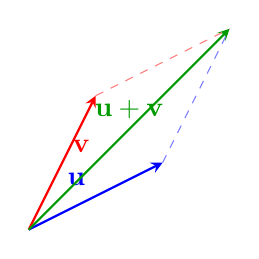
\begin{tikzpicture}[scale=0.85, >=stealth]
        \draw[->, thick, blue] (0, 0) -- (2, 1) node[midway, above left] {$\mathbf{u}$};
        \draw[->, thick, red] (0, 0) -- (1, 2) node[midway, above right] {$\mathbf{v}$};
        \draw[->, thick, green!60!black] (0, 0) -- (3, 3) node[midway, above] {$\mathbf{u} + \mathbf{v}$};
        
        \draw[dashed, blue!50] (2, 1) -- (3, 3);
        \draw[dashed, red!50] (1, 2) -- (3, 3);
      \end{tikzpicture}
      \caption{Addition is visualized using the ``parallelogram rule.''}
      \label{fig:vector-addition}
    \end{subfigure}
    \begin{subfigure}[b]{0.48\textwidth}
      \centering
      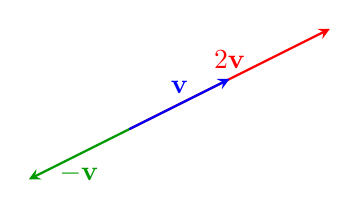
\begin{tikzpicture}[scale=0.85, >=stealth]
        \draw[->, thick, red] (0, 0) -- (3, 1.5) node[midway, above] {$2\mathbf{v}$};
        \draw[->, thick, blue] (0, 0) -- (1.5, 0.75) node[midway, above] {$\mathbf{v}$};
        \draw[->, thick, green!60!black] (0, 0) -- (-1.5, -0.75) node[midway, below] {$-\mathbf{v}$};
      \end{tikzpicture}
      \caption{Scalar multiplication is simply an stretch of the vector.}
      \label{fig:scalar-multiplication}
    \end{subfigure}
  \end{figure}

  The other interpretation is to simply see it as a tuple of numbers, which is useful when dealing with arbitrary dimensions. This interpretation is more suited to the intuition of a computer scientist, who can interpret vectors as arrays with element-wise operations. 

  \begin{figure}[H]
    \centering
    \begin{subfigure}[b]{0.48\textwidth}
      \centering
      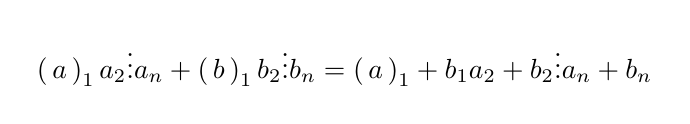
\begin{tikzpicture}[scale=0.9, >=stealth]
        \node at (0, 0.3) {
          $\begin{pmatrix}
            a_1 \\
            a_2 \\
            \vdots \\
            a_n
          \end{pmatrix}
          +
          \begin{pmatrix}
            b_1 \\
            b_2 \\
            \vdots \\
            b_n
          \end{pmatrix}
          =
          \begin{pmatrix}
            a_1 + b_1 \\
            a_2 + b_2 \\
            \vdots \\
            a_n + b_n
          \end{pmatrix}$
        };
      \end{tikzpicture}
      \caption{Addition is done component-wise.}
      \label{fig:tuple-addition}
    \end{subfigure}
    \hfill 
    \begin{subfigure}[b]{0.48\textwidth}
      \centering
      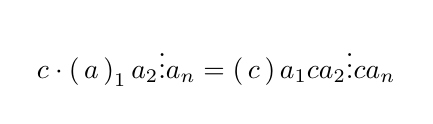
\begin{tikzpicture}[scale=0.9, >=stealth]
        \node at (0, 0.3) {
          $c \cdot
          \begin{pmatrix}
            a_1 \\
            a_2 \\
            \vdots \\
            a_n
          \end{pmatrix}
          =
          \begin{pmatrix}
            c a_1 \\
            c a_2 \\
            \vdots \\
            c a_n
          \end{pmatrix}$
        };
      \end{tikzpicture}
      \caption{Scalar multiplication is done component-wise.}
      \label{fig:tuple-scalar}
    \end{subfigure}
    \caption{}
  \end{figure}

  By introducing a coordinate basis (also called a frame), we can unify the two interpretations above by decomposing each arrow into its component vectors, with magnitudes equal to the elements of the corresponding tuple. There are other ways that vectors are introduced.\footnote{Aspinwall mentioned that there are 4 or 5 ways? Another being in terms of derivations?} Mathematicians try to unify the two\footnote{similar to what 3Blue1Brown says in his Linear Algebra Youtube series.} by generalizing both of these interpretations into the following definition. 

  \begin{definition}[Vector Space]
    A \textbf{vector space $V$ over a field $\mathbb{F}$} is a set endowed with two operations---addition $+: V \times V \to V$ and scalar multiplication $\cdot: \mathbb{F} \times V \to V$. It satisfies the following properties. 
    \begin{enumerate}
      \item \textit{Group Structure}. $(V, +)$ is an abelian group. 
      \item \textit{Scalar Distributivity}. For $\lambda, \mu \in \mathbb{F}$ and $v, u \in V$, $(\lambda + \mu) v = \lambda v + \mu v$
      \item \textit{Vector Distributivity}. For $\lambda \in \mathbb{F}$ and $v, u \in V$, $\lambda (v + u) = \lambda v + \lambda u$
      \item \textit{Associativity of Scalar Multiplication}. For $\lambda, \mu \in \mathbb{F}$ and $v \in V$, $(\lambda \mu) v = \lambda (\mu v) = \mu (\lambda v)$ 
    \end{enumerate}
    A \textbf{vector} is an element of a vector space.
  \end{definition} 

  We define some more vector spaces that are often used. 

  \begin{example}[$\mathbb{R}^n$]
    The set of all $n$-tuples of real numbers $\mathbb{R}^n = \{(a_1, \dots, a_n) : a_i \in \mathbb{R}\}$ forms a vector space over $\mathbb{R}$ with component-wise addition and scalar multiplication. This is the foundational setting for analytic geometry, physics (mechanics, electromagnetism), engineering, computer graphics, machine learning, and economics.
  \end{example}

  \begin{example}[$\mathbb{C}^n$]
    The set of all $n$-tuples of complex numbers $\mathbb{C}^n = \{(a_1, \dots, a_n) : a_i \in \mathbb{C}\}$ forms a vector space over $\mathbb{C}$ (and also over $\mathbb{R}$, with dimension $2n$). Essential in quantum mechanics, signal processing (Fourier analysis), electrical engineering, and solving differential equations.
  \end{example}

  \begin{example}[$\mathbb{Z}_p^n$]
    The set of all $n$-tuples of elements in the finite field $\mathbb{Z}_p = \{0, 1, \dots, p-1\}$ (with $p$ prime) forms a vector space over $\mathbb{Z}_p$ with component-wise operations. Central to cryptography (elliptic curve cryptography, Reed-Solomon codes), coding theory, and computer science.
  \end{example}

  \begin{example}[Function Space]
    Let $X$ be any set. The set of all functions $f: X \to \mathbb{F}$ from $X$ to a field $\mathbb{F}$ forms a vector space over $\mathbb{F}$ with pointwise addition $(f+g)(x) = f(x) + g(x)$ and scalar multiplication $(c \cdot f)(x) = c \cdot f(x)$. The foundational object of functional analysis; appears in probability theory (random variables), signal processing, and differential equations.
  \end{example}

  \begin{example}[Continuous Functions]
    The set $C(I)$ of all continuous real-valued functions on an interval $I \subset \mathbb{R}$ forms a vector space over $\mathbb{R}$ with pointwise operations. Fundamental in real analysis, differential equations, Fourier series, and physics (modeling continuous phenomena).
  \end{example}

  \begin{example}[Polynomials of Finite Degree]
    The set of all polynomials of degree strictly less than $n$ with coefficients in $\mathbb{F}$ defines a vector space over $\mathbb{F}$. Widely used in numerical analysis (interpolation), approximation theory, and signal processing.
  \end{example}

  \begin{example}[Sequence Space $\ell^p$]
    The set of all sequences $(a_1, a_2, \dots)$ of elements in $\mathbb{F}$ such that $\sum_{i=1}^\infty |a_i|^p < \infty$ forms a vector space over $\mathbb{F}$ for $1 \leq p < \infty$. Core example in functional analysis; arises in statistics (finite variance sequences), signal processing, and probability theory.
  \end{example}

  The examples above should convince you that linear algebra is fundamental in almost every quantitative field, to the point where it should be considered universal knowledge.  

  \begin{theorem}[No Zero Divisors]
    There are no zero divisors of vector space $V$. That is, 
    \begin{equation}
      \lambda v = 0 \implies \lambda = 0 \text{ or } v = 0
    \end{equation}
  \end{theorem}
  \begin{proof}
    $\lambda v = 0 \implies \lambda v + \lambda v = 0 + \lambda v \implies 2\lambda v = \lambda v \implies (2\lambda - \lambda ) v = 0$. But $\lambda \neq 0$, so $v$ must equal $0$. This leads to a contradiction. 
  \end{proof} 

  Now we move onto the other primary object of study: the linear map. 

  \begin{definition}[Linear Map]
    Given vector spaces $V, W$ over the same field $\mathbb{F}$, a function $T: V \longrightarrow W$ is called a \textbf{linear map} if it satisfies the following linearity properties: 
    \begin{equation}
      T(v_1 + v_2) = T(v_1) + T(v_2), \quad T(c v) = c T(v)
    \end{equation}
    for all $v_1, v_2 \in V, c \in \mathbb{F}$. 

    \begin{figure}[H]
      \centering 
      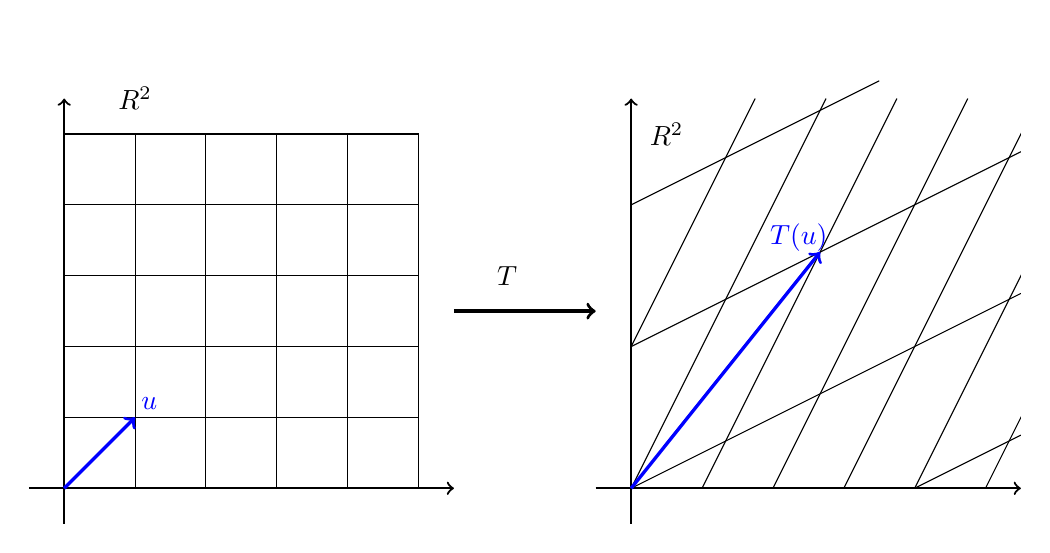
\begin{tikzpicture}[scale=0.9]
        % Left grid (domain)
        \begin{scope}[shift={(-5,0)}]
          % Draw grid
          \draw[step=1cm, black] (0,0) grid (5,5);
          
          % Draw axes
          \draw[thick, ->] (-0.5,0) -- (5.5,0);
          \draw[thick, ->] (0,-0.5) -- (0,5.5);
          
          % Label the space
          \node at (1,5.5) {$\mathbb{R}^2$};
          \draw[->, very thick, blue] (0, 0) -- (1, 1);
          \node[blue] at (1.2,1.2) {$u$};
        \end{scope}
        
        % Transformation arrow
        \draw[->, very thick] (0.5,2.5) -- (2.5,2.5);
        \node at (1.25,3) {$T$};

        
        % Right grid (codomain)
        \begin{scope}[shift={(3,0)}]
          % Draw only axes
          \draw[thick, ->] (-0.5,0) -- (5.5,0);
          \draw[thick, ->] (0,-0.5) -- (0,5.5);
          
          % Label the space
          \node at (0.5,5) {$\mathbb{R}^2$};
          
          % Clip all drawing to stay within visible area
          \begin{scope}
            \clip (-0.5,-0.5) rectangle (5.5,6.5);
            
            % Existing lines with slope 1/2
            \draw[] (4,0) -- (5.5,0.75);
            \draw[] (0,0) -- (5.5,2.75);
            \draw[] (0,2) -- (5.5,4.75);
            \draw[] (0,4) -- (3.5,5.75);
            
            % New lines with slope 2
            \draw[] (5,0) -- (7.75,5.5);
            \draw[] (4,0) -- (6.75,5.5);
            \draw[] (3,0) -- (5.75,5.5);
            \draw[] (2,0) -- (4.75,5.5);
            \draw[] (1,0) -- (3.75,5.5); 
            \draw[] (0,0) -- (2.75,5.5); 
            \draw[] (0,2) -- (1.75,5.5); 
          \end{scope}
          \node[blue] at (2.366,3.533) {$T(u)$};
          \draw[->, very thick, blue] (0, 0) -- (2.666, 3.333);
        \end{scope}
      \end{tikzpicture}
      \caption{A great way to visualize this is that linear maps transform \textit{lines to lines}. That is, we can think of the grid moving in a uniform way so that all squares become parallelograms. 3Blue1Brown has a really nice animation in his Linear Algebra Youtube Series.}
      \label{fig:linear_map}
    \end{figure}
  \end{definition}

  \begin{definition}[Isomorphism]
    If a linear map $T: V \to W$ is called a \textbf{(vector space) isomorphism} if $T$ is bijective. In this case, $T^{-1}$ is also a linear map. Then, we say $V$ is \textbf{isomorphic} to $W$, denoted $V \simeq W$. 
  \end{definition}
  \begin{proof}
    It suffices to show that bijection $\iff$ the inverse is linear. 
  \end{proof}

  Following the terminology in algebra, we sometimes call a linear map $T: V \to V$ an \textit{endomorphism} and an isomorphism $T: V \to V$ an \textit{automorphism}. 

\subsection{Basis and Dimension}

  While there are a lot of things we can do with the axioms themselves, it is often convenient to add in a bit of structure to our vector space. First, note that we can write out vectors as sums of other vectors. 

  \begin{definition}[Linear Combination]
    Given vector space $V$, a \textbf{linear combination} of a finite\footnote{We restrict ourselves to the finite case since we do not know how to evaluate series yet.} number of vectors $v_1, v_2, \ldots, v_n \in V$ is a vector of the form 
    \begin{equation}
      v = c_1 v_1 + c_2 v_2 + \ldots + c_n v_n
    \end{equation}
    where $c_1, \ldots, c_n \in \mathbb{F}$. 
  \end{definition}

  \begin{definition}[Span]
    The \textbf{span} of a collection of vectors $v_1, v_2, \ldots, v_n \in V$ is defined in the following equivalent ways: 
    \begin{enumerate}
      \item \textit{Smallest Subspace}. It is the intersection of all subspaces $W \subset V$ that each contains all $v_1, \ldots, v_n$.\footnote{This is the more general definition and extends to the infinite-dimensional case.}
      \item \textit{Set of Linear Combinations}. It is the subspace of vectors defined 
        \begin{equation}
          \Span \{ v_1, v_2, \ldots, v_n \} \coloneqq \{ c_1 v_1 + c_2 v_2 + \ldots + c_n v_n \mid  c_1, \ldots, c_n \in \mathbb{F}\}
        \end{equation}
    \end{enumerate}
  \end{definition}
  \begin{proof}
    
  \end{proof}

  It clearly follows that $v_1, \ldots, v_n$ span the whole space $V$ if every vector in $V$ can be expressed as a linear combination of the $v_i$'s. 

  \begin{definition}[Linear Independence]
    Vectors $v_1, \ldots, v_n$ are 
    \begin{enumerate}
      \item \textbf{linearly independent} if 
        \begin{equation}
          c_1 v_1 + c_2 v_2 + c_3 v_3 + \ldots + c_n v_n = 0 \implies c_1, \ldots, c_n = 0
        \end{equation}
      \item \textbf{linearly dependent} if it is not linearly independent, i.e. there exists some $1 \leq i \leq n$ such that $v_i$ is in the span of vectors $v_1, \ldots, v_{i-1}, v_{i+1}, \ldots, v_n$. 
    \end{enumerate}
  \end{definition}

  \begin{definition}[Basis]
    A set of linearly independent vectors $v_1, \ldots, v_n$ that span vector space $V$ is called a \textbf{basis} of $V$. These vectors $v_i$ are called \textbf{basis vectors}. Note that this basis is not unique; it is actually highly un-unique. 
  \end{definition}

  \begin{example}[Standard Basis]
    The basis $e_i$ of $\mathbb{F}^n$ are the vectors with every element equal to $0$ except for the $i$th element, which is equal to $1$. 
  \end{example}

  \begin{theorem}[Maximally Independent Set is a Basis]
    Let $V$ be a vector space and $S$ be a subset of $V$ (not necessarily a subspace). Then, any maximal linearly independent subset $\{ e_1, e_2, \ldots, e_k\}$ of a set $S$ is a basis of $\Span S$. 
  \end{theorem}

  \begin{definition}[Dimension]
    The number of vectors in any basis of vector space $V$ is called the \textbf{dimension} of $V$, denoted $\dim{V}$. 
  \end{definition}
  \begin{proof}
    We must show that this is well defined by proving that every possible basis of a vector space $V$ has the same number of vectors.
  \end{proof}

  \begin{theorem}[Isomorphism to $\mathbb{F}^n$]
    Every $n$-dimensional vector space $V$ over $\mathbb{F}$ is isomorphic to $\mathbb{F}^n$, the set of $n$-tuples of elements in $\mathbb{F}$. 
  \end{theorem}

  \begin{corollary}[Isomorphism Between $n$-Dimensional Vector Spaces]
    Finite-dimensional vector spaces of the same field are isomorphic if and only if their dimensions are the same. 
  \end{corollary}

  \begin{example}
    The field of complex numbers $\mathbb{C}$, regarded as a vector space over $\mathbb{R}$, has dimension $2$. 
  \end{example}

\subsection{Subspaces}

  \begin{definition}[Subspace]
    Given vector space $V$, A subset $W \subset V$ is a \textbf{subspace} if sums and scalar multiples of elements of $W$ belong to $W$. 
  \end{definition}

  Note that $\{ 0 \}, V$ are subspaces of $V$. Regarding notation, when we write $W \subset V$ from now on, this is in the subspace sense, and not the set-theoretic subset. 

  \begin{definition}[Hyperplane]
    A $(n - 1)$-dimensional subspace of an $n$-dimensional space is called a \textbf{hyperplane}. 
  \end{definition}

  \begin{definition}[Sum of Subspaces]
    The \textbf{sum of subspaces} $U_1, U_2, \ldots, U_n \subset V$ is defined 
    \begin{equation}
      \sum_{i=1}^n U_i \coloneqq \Big\{ \sum_{i = 1}^n u_i \mid u_i \in U_i\Big\}
    \end{equation}
    That is, it is the set of all vectors that can be expressed as the sum of vectors in each of its respective space. 
  \end{definition}

  \begin{definition}[Direct Sum of Spaces]
    Given subspaces $U_1, \ldots, U_n \subset V$, if $V_i$'s are pairwise disjoint---except at the origin---then we call their sum the \textbf{direct sum}. 
    \begin{equation}
      \bigoplus_{i=1}^n V_i \equiv \Big\{ \sum_{i=1}^n v_i \; | \; v_i \in V_i\Big\}
    \end{equation}
    It is a vector space where each vector can be expressed uniquely as the sum of vectors in each respective subspace. 
  \end{definition}
  \begin{proof}
    
  \end{proof}

  The crucial difference between the sum and the direct sum is that the direct sum requires the subspaces to be disjoint except for at the origin, which allows the expression of each vector in $V_1 \oplus \ldots \oplus V_n$ to be unique. It is also worth noting that the Cartesian product of vector spaces is merely just the set of tuples of vectors that are in each respective space and is \textit{not} a vector space (since addition and multiplication is not defined on that new set). If we define the operations component-wise, then 
  \begin{equation}
    \prod_{i=1}^n V_i = \sum_{i=1}^n V_i
  \end{equation}

  \begin{example}[Vector Space as Direct Sum of Basis]
    Note that we can also define the direct sum of spaces $U$ and $V$ by their basis. That is, given that the basis for $U$ is $\{e_i\}_{i=1}^n$ and the basis for $V$ is $\{f_j\}_{j=1}^n$, the basis for $U \oplus V$ is
    \begin{equation}
      \{(e_1, 0), (e_2, 0), \ldots, (e_n, 0), (0, f_1), \ldots, (0, f_m)\}
    \end{equation}
  \end{example}

  \begin{example}[Complex Vector Spaces as Real Vector Spaces]
    Vector spaces over one field can be interpreted as a vector space over another field. This is most common when interpreting complex vector spaces as real ones. For example, given a complex vector space $Z$ with basis $\{z_1, z_2, \ldots, z_n\}$, every vector can be expressed as
    \begin{equation}
      z = \sum_{j=1}^n c_j z_j, \; c_j \in \mathbb{C}
    \end{equation}
    We can set $c_j = a_j + b_j i$ uniquely, with $a, b \in \mathbb{R}$, and rewrite
    \begin{equation}
      z = \sum_{j=1}^n a_j z_j + b_j (i z_j)
    \end{equation}
    $\implies \{ z_j\} \cup \{ i z_j\}$ forms a basis of $Z$ as a \textit{real vector space}. 
  \end{example}

  \begin{theorem}[Dimension of Direct Sum]
    The dimension of the direct sum of vector spaces is 
    \begin{equation}
      \dim{\bigoplus_{i=1}^n V_i} = \sum_{i=1}^n \dim{V_i}
    \end{equation}
  \end{theorem}
  \begin{proof}
    This follows from the basis construction of the direct sum of $V_i$'s. 
  \end{proof}

  \begin{definition}[Congruence Relations on Vector Spaces]
    Given vector space $V$ and subspace $W \subset V$ we say that two vectors $v_1, v_2 \in V$ are \textbf{congruent modulo $W$}, denoted $v_1 \equiv v_2 \pmod{W}$, if $v_2 - v_1 \in W$. This is a congruence relation. 
  \end{definition}
  \begin{proof}
    It remains to prove that $\equiv$ is a congruence relation. The congruence classes $\{ y\}$ is the set of all vectors that are congruent modulo $W$ to $y$. 
  \end{proof}

  \begin{definition}[Quotient Vector Space]
    The \textbf{quotient (vector) space} $V$ modulo $W$, denoted $V/W$, is the set of all congruence classes modulo $W$. We can define addition and scalar multiplication on this set as such 
    \begin{equation}
      [x] + [y] = [x + y]
    \end{equation}
  \end{definition}

  \begin{theorem}[Decomposition into Subspace and Quotient Space]
    Given vector space $V$, $W$ a subspace of $V$. Then, 
    \begin{equation}
      V \simeq W \oplus \frac{V}{W}
    \end{equation}
  \end{theorem}
  \begin{proof}
    
  \end{proof}

\subsection{Dual Spaces}

  Now we talk about dual spaces, which are nice since their construction and existence doesn't require us to have any structure on the vector space. 

  \begin{definition}[Dual Space]
    Given a vector space $V$ over $\mathbb{F}$, the \textbf{dual vector space} $V^\dagger$ is defined as the vector space of linear maps $\ell: V \to \mathbb{F}$. Given $\ell_1, \ell_2 \in V^\dagger$, $v \in V$, and $c \in \mathbb{F}$, we define
    \begin{enumerate}
      \item \textit{Addition}. $(\ell_1 + \ell_2)(v) = \ell_1 (v) + \ell_2 (v)$. 
      \item \textit{Scalar Multiplication}. $(c \ell_1)(v) = c \ell_1 (v)$. 
    \end{enumerate}
  \end{definition}
  \begin{proof}
    We must prove that this is indeed a vector space. 
  \end{proof}

  As the name suggests, we call the vectors of the dual space as \textit{dual vectors}. Often, mathematicians will call them \textit{functionals}, since usually the base space $V$ is a vector space of functions, and functionals are mappings that act on functions. Analysis of this in the infinite-dimensional case requires much more machinery, so we will focus on the finite-dimensional case. 

  \begin{theorem}[Dimensions of Dual of Finite-Dimensional Vector Spaces]
    Let $V$ be a finite-dimensional vector space and $V^\ast$ its dual. Then, 
    \begin{equation}
      \dim{V} = \dim{V^\dagger}
    \end{equation}
  \end{theorem}
  \begin{proof}
    
  \end{proof}

  \begin{definition}[Dual Basis]
    Given a basis $\{ e_1, e_2, \ldots, e_n\}$ of $V$, the \textbf{dual basis} $\{f_1, f_2, \ldots, f_n\}$ of $V^\dagger$ has vectors satisfying 
    \begin{equation}
      f_j (e_i) = \delta_{i j} = 
      \begin{cases}
      0 & i \neq j \\
      1 & i = j
      \end{cases}
    \end{equation}
    where $\delta_{i j}$ is called the \textbf{Kronecker delta function}. 
  \end{definition}

  While we initially view elements of $V$ as "things" and elements of $V^\dagger$ as linear functions, this thought is actually erroneous. Given $l \in V^\dagger$, we see that 
  \begin{equation}
    l: V \longrightarrow \mathbb{F}
  \end{equation}
  But since both $V$ and $V^\dagger$ are vector spaces, we can also see that given $x \in V$, $x$ is also a linear function 
  \begin{equation}
    x: V^\dagger \longrightarrow \mathbb{F}, \text{ where } x(l) \equiv l(x)
  \end{equation}
  But this means that $x$ is an element of $V^{\dagger\dagger}$ the dual of $V$! This statement is elaborated with the following theorem. 

  \begin{theorem}[Canonical Isomorphisms of Double Duals]
    $V^{\dagger\dagger}$ is \textbf{naturally isomorphic}\footnote{What we mean by natural is that we do not need to select a basis in either vector space to define the isomorphism. } to vector space $V$. 
  \end{theorem}
  \begin{proof}
    We fix a vector $l \in V^\dagger$, and given $x \in V, \phi \in V^{\dagger\dagger}$, we define
    \begin{equation}
      \phi(l) \coloneqq l(x)
    \end{equation}
    This defines a one-to-one correspondence between $V$ and $V^{\dagger\dagger}$. 
  \end{proof}

  On the contrary, there is no way to define an isomorphism between $V$ and $V^\dagger$ without further structure on $V$. In conclusion, this theorem tells us that it is important to be aware of this \textit{duality} between elements $x \in V$ and $l \in V^\dagger$, and thus we should interpret $x \in V$ as a linear function of $V^\dagger$ and $l \in V^\dagger$ as a linear function of $V$.

  \begin{definition}[Annihilator]
    Let $W$ be a subspace of $V$. Then the set of functions in $V^\dagger$ that vanish on $W$, that is, satisfy
    \begin{equation}
      l(w) = 0 \text{ for all } w \in W
    \end{equation}
    is called the \textbf{annihilator} of $W$, denoted $W^0$. If $W = V$, then it is easy to see that $W^0$ is trivial. 
  \end{definition}

  \begin{theorem}[Annihilator and Dual Quotient Space]
    Let $V$ be a vector space and $W \subset V$. Then, 
    \begin{enumerate}
      \item $W^0 \simeq (V/W)^\dagger$
      \item $\dim W^0 + \dim W = \dim V$ 
      \item $W^{00} = W$. 
    \end{enumerate}
  \end{theorem}
  \begin{proof}
    Listed. 
    \begin{enumerate}
      \item The isomorphism is defined as such. Given $l \in W^0$, we define $L \in (V/W)^\dagger$ as 
        \begin{equation}
          L\{x\} \equiv l(x)
        \end{equation}
    \end{enumerate}
  \end{proof}

  \begin{theorem}[Quadrature Formula]
    Let $l$ be an interval on $\mathbb{R}$ containing $t_1, t_2, \ldots, t_n$ $n$ distinct points. Then, given any polynomial $p$ with degree $< n$, there exist $n$ real numbers $c_1, c_2, \ldots, c_n$ such that
    \begin{equation}
      \int_l p(t) d t = c_1 p(t_1) + c_2 p(t_2) + \ldots + c_n p(t_n)
    \end{equation}
    called the \textit{quadrature formula} suffices. That is, the integral of any polynomial over $l$ can be expressed as a linear combination of the polynomials evaluated at $n$ distinct points in $l$. 
  \end{theorem}
  \begin{proof}
    The space of all polynomials with degree $< n$ is an $n$-dimensional vector space, denote it $V$. We define the basis of the dual space $V^\dagger$ as 
    \begin{equation}
      \phi_i (p) \equiv p(t_i), \; i = 1, 2, \ldots, n
    \end{equation}
    with addition and scalar multiplication defined
    \begin{align*}
      & (\phi + \gamma) (p) \equiv \phi(p) + \gamma(p) \\
      & (c \phi) (p) \equiv c \phi (p) 
    \end{align*}
    We can see that the $\phi$'s are indeed linear since, given $p, q \in \mathbb{R}[t]$
    \begin{align*}
      & \phi_i (p + q) = (p + q) (t_i) = p(t_i) + q(t_i) = \phi_i (p) + \phi_i (q) \\
      & \phi_i (c p) = (c p) (t_i) = c p(t_i) = c \phi_i (p)
    \end{align*}
    We claim that all the $phi_i$'s are linearly independent. Assume that 
    \begin{equation}
      \sum_{i=1}^n c_i \phi_i (p) = \sum_{i=1}^n c_i p(t_i) = 0
    \end{equation}
    Since the $\phi$'s must be linearly independent for every polynomial $p$, set it equal to
    \begin{equation}
      q_k (t) \equiv \prod_{j \neq k} (t - t_j), \; k = 1, 2, \ldots, n
    \end{equation}
    $p = q_k$ must imply that all $\phi_i (p) = 0$ for all $i \neq k$, which implies that $c_k = 0$ in the linear combination. Repeating this for $k = 1, 2, \ldots, n$ results in all $c_i = 0$, implying that the $\phi_i$'s form a basis of $V^\dagger$. Clearly, the function of definite integration over $l$ is a linear mapping from $V \longrightarrow \mathbb{R}$, meaning that it is in $V^\dagger$. Therefore, it can be expressed as a linear combination of $\phi_i$'s. 
  \end{proof}

\subsection{Exercises} 

  \begin{exercise}[Lax 1.1] 
    Show that the zero of vector addition is unique.
  \end{exercise}

  \begin{exercise}[Lax 1.2] 
    Show that the vector with all components zero serves as the zero element of classical vector addition.
  \end{exercise}

  \begin{exercise}[Lax 1.3] 
    Show that (i) and (iv) are isomorphic.
  \end{exercise}

  \begin{exercise}[Lax 1.4] 
    Show that if $S$ has $n$ elements, (i) and (iii) are isomorphic.
  \end{exercise}

  \begin{exercise}[Lax 1.5] 
    Show that when $K = \mathbb{R}$, (iv) is isomorphic with (iii) when $S$ consists of $n$ distinct points of $\mathbb{R}$.
  \end{exercise}

  \begin{exercise}[Lax 1.6] 
    Denote by $X$ the linear space of all polynomials $p(t)$ of degree $< n$, and denote by $Y$ the set of polynomials that are zero at $t_1,\ldots,t_j$, $j < n$.
    (i) Show that $Y$ is a subspace of $X$.
    (ii) Determine dim $Y$.
    (iii) Determine dim $X/Y$.
  \end{exercise}

  \begin{exercise}[Lax 1.7] 
    Prove (i)-(iii) above. Show furthermore that if $x_1 \equiv x_2$, then $kx_1 \equiv kx_2$ for every scalar $k$.
  \end{exercise}

  \begin{exercise}[Lax 1.9] 
    Show that the set of all linear combinations of $x_1,\ldots,x_j$ is a subspace of $X$, and that it is the smallest subspace of $X$ containing $x_1,\ldots,x_j$. This is called the subspace spanned by $x_1,\ldots,x_j$.
  \end{exercise}

  \begin{exercise}[Lax 1.10] 
    Show that if the vectors $x_1,\ldots,x_j$ are linearly independent, then none of the $x_i$ is the zero vector.
  \end{exercise}

  \begin{exercise}[Lax 1.15] 
    Show that the above definition of addition and multiplication by scalars is independent of the choice of representatives in the congruence class.
  \end{exercise}

  \begin{exercise}[Lax 1.11] 
    Prove that if $X$ is finite dimensional and the direct sum of $Y_1,\ldots,Y_m$, then
    \[ \dim X = \sum \dim Y_j. \]
  \end{exercise}

  \begin{exercise}[Lax 1.12] 
    Show that every finite-dimensional space $X$ over $K$ is isomorphic to $K^n$, $n = \dim X$. Show that this isomorphism is not unique when $n$ is $>1$.
  \end{exercise}

  \begin{exercise}[Lax 1.14] 
    Show that two congruence classes are either identical or disjoint.
  \end{exercise}

  \begin{exercise}[Lax 1.18] 
    Show that
    \[ \dim X_1 \oplus X_2 = \dim X_1 + \dim X_2. \]
  \end{exercise}

  \begin{exercise}[Lax 1.19] 
    $X$ a linear space, $Y$ a subspace. Show that $Y \oplus X/Y$ is isomorphic to $X$.
  \end{exercise}

  \begin{exercise}[Lax 1.17] 
    Prove Corollary 6': A subspace $Y$ of a finite-dimensional linear space $X$ whose dimension is the same as the dimension of $X$ is all of $X$.
  \end{exercise}

  \begin{exercise}[Lax 2.1] 
    Given a nonzero vector $x_1$ in $X$, show that there is a linear function $l$ such that 
  \end{exercise}

  \begin{exercise}[Lax 2.2] 
    Verify that $Y^\perp$ is a subspace of $X'$.
  \end{exercise}

  \begin{exercise}[Lax 2.3] 
    Prove Theorem 6: Denote by $Y$ the smallest subspace containing $S$:
    \[S^\perp = Y^\perp.\]
  \end{exercise}

  \begin{exercise}[Lax 2.4] 
    In Theorem 6 take the interval $I$ to be $[-1, 1]$, and take $n$ to be 3. Choose the three points to be $t_1 = -a$, $t_2 = 0$, and $t_3 = a$.
    
    \begin{enumerate}
      \item[(i)] Determine the weights $m_1, m_2, m_3$ so that (9) holds for all polynomials of degree $<3$.
      \item[(ii)] Show that for $a > \sqrt{1/3}$, all three weights are positive.
      \item[(iii)] Show that for $a = \sqrt{3/5}$, (9) holds for all polynomials of degree $<6$.
    \end{enumerate}
  \end{exercise}

  \begin{exercise}[Lax 2.5] 
    In Theorem 6 take the interval $I$ to be $[-1, 1]$, and take $n$ to be 4. Choose the four points to be $-a, -b, b, a$.
    
    \begin{enumerate}
      \item[(i)] Determine the weights $m_1, m_2, m_3$, and $m_4$ so that (9) holds for all polynomials of degree $<4$.
      \item[(ii)] For what values of $a$ and $b$ are the weights positive?
    \end{enumerate}
  \end{exercise}

  \begin{exercise}[Lax 2.6] 
    Let $\mathcal{P}_2$ be the linear space of all polynomials
    \[p(x) = a_0 + a_1x + a_2x^2\]
    
    with real coefficients and degree $\leq 2$. Let $\xi_1, \xi_2, \xi_3$ be three distinct real numbers, and then define
    \[\ell_j = p(\xi_j) \quad \text{for} \quad j = 1,2,3.\]
    
    \begin{enumerate}
      \item[(a)] Show that $\ell_1, \ell_2, \ell_3$ are linearly independent linear functions on $\mathcal{P}_2$.
      \item[(b)] Show that $\ell_1, \ell_2, \ell_3$ is a basis for the dual space $\mathcal{P}_2'$.
      \item[(c)] 
        \begin{enumerate}
          \item[(1)] Suppose $\{e_1, \ldots, e_n\}$ is a basis for the vector space $V$. Show there exist linear functions $\{\ell_1, \ldots \ell_n\}$ in the dual space $V'$ defined by
          \[\ell_i(e_j) = \begin{cases} 1 & \text{if } i = j, \\ 0 & \text{if } i \neq j. \end{cases}\]
        
          Show that $\{\ell_1, \ldots, \ell_n\}$ is a basis of $V'$, called the \textit{dual basis}.
          \item[(2)] Find the polynomials $p_1(x), p_2(x), p_3(x)$ in $\mathcal{P}_2$ for which $\ell_1, \ell_2, \ell_3$ is the dual basis in $\mathcal{P}_2'$.
        \end{enumerate}
    \end{enumerate}
  \end{exercise}

  \begin{exercise}[Lax 2.7] 
    Let W be the subspace of $\mathbb{R}^4$ spanned by $(1, 0, -1, 2)$ and $(2, 3, 1, 1)$.
    Which linear functions $\ell(x) = c_1x_1 + c_2x_2 + c_3x_3 + c_4x_4$ are in the annihilator of W?
  \end{exercise}

  \begin{exercise}[Math 403 Spring 2020, Week 1.2] 
    If $e_1, e_2, \ldots, e_n$ is a basis for $V$ and we define linear maps $e_i^\prime$ to $K$ by
    \[e_i^\prime(e_j) = \delta_{ij},\]
    
    then prove $e_1^\prime, e_2^\prime, \ldots, e_n^\prime$ form a basis for $V^\prime$.
  \end{exercise}

  \begin{exercise}[Math 403 Spring 2020, Week 4.2] 
    Find the Jordan Normal Form, $J$, of
    \[A = \begin{pmatrix} 
      4 & -2 & -6 \\
      -1 & 2 & 2 \\
      1 & -1 & -1
    \end{pmatrix}\]
    
    and a matrix $S$ such that $J = S^{-1}AS$.
  \end{exercise}

  \begin{exercise}[Math 403 Spring 2020, Week 4.3] 
    Let $d^n(\alpha)$ denote the dimension of the nullspace of $(\alpha I - A)^n$ for a matrix $A$ and a scalar $\alpha$. In the following examples we list all the possible nonzero values of $d^n(\alpha)$. In each case find the Jordan Normal Form of $A$ or prove $A$ cannot exist.
    \begin{enumerate}
      \item $d^1(1) = 2$, and $d^n(1) = 3$ if $n \geq 2$.
      \item $d^n(2) = 1$ if $n \geq 1$; $d^1(1) = 2$, $d^n(1) = 4$ if $n \geq 2$.
      \item $d^1(1) = 1$, $d^n(1) = 3$ if $n \geq 2$.
    \end{enumerate}
  \end{exercise}

  \begin{exercise}[Math 403 Spring 2020, Week 7.1] 
    Let
    \[\sigma_x = \begin{pmatrix} 0 & 1 \\ 1 & 0 \end{pmatrix}, \quad
    \sigma_y = \begin{pmatrix} 0 & i \\ -i & 0 \end{pmatrix}, \quad
    \sigma_z = \begin{pmatrix} 1 & 0 \\ 0 & -1 \end{pmatrix}.\]
    
    Compute $\Delta(\sigma_x)\Delta(\sigma_y)$ if the state vector is $\begin{pmatrix} 1 \\ 0 \end{pmatrix}$. Is this consistent with the Heisenberg Uncertainty Principle?
  \end{exercise}

  \begin{exercise}[Math 403 Spring 2020, Week 8.1] 
    Compute the singular value decompositions of the following matrices
    \begin{enumerate}
      \item $(1 \quad 1)$
      
      \item $\begin{pmatrix} 1 & 1 \\ 0 & 1 \end{pmatrix}$
      
      \item $\begin{pmatrix} 0 & 1 \\ -1 & 0 \end{pmatrix}$
    \end{enumerate}
  \end{exercise}

  \begin{exercise}[Math 403 Spring 2020, Week 8.2] 
    Let $M$ be any matrix over $\mathbb{R}$ and let $M^{(k)}$ be the rank $k$ approximation of $M$ we did in class. That is $M^{(k)}$ is obtained from an SVD of $M$ where we set all but the $k$ largest singular values to 0.
    \begin{enumerate}
      \item Show that $B = M^{(k)}$ is not the \textit{unique} matrix that minimizes the norm
      \[||M-B||_2\]
      if $\sigma_k = \sigma_{k+1}$ where $\sigma_1 \geq \sigma_2 \geq \cdots$ are the singular values of $M$.
      
      \item Discuss if $B = M^{(k)}$ is the unique matrix that minimizes this norm if $\sigma_k > \sigma_{k+1}$.
    \end{enumerate}
  \end{exercise}

  \begin{exercise}[Math 403 Spring 2020, Week 9.1] 
    Let
    \[A = \begin{pmatrix} 
      0 & 0 & 0 & 1/3 \\
      1/2 & 0 & 1 & 1/3 \\
      0 & 1 & 0 & 1/3 \\
      1/2 & 0 & 0 & 0
    \end{pmatrix}.\]
    
    Compute the asymptotic behaviour of $A^N v$ where $v$ has coordinates $(1/4, 1/4, 1/4, 1/4)$ and $N$ is large.
  \end{exercise}

  \begin{exercise}[Math 403 Spring 2020, Week 10.1] 
    Prove $v \otimes 0 = 0$ in $V \otimes V$ for any vector $v \in V$.
  \end{exercise}

  \begin{exercise}[Math 403 Spring 2020, Week 10.2] 
    Prove there is a natural isomorphism between the vector spaces $\text{Hom}(V,V)$ and $V \otimes V^*$.
  \end{exercise}

  \begin{exercise}[Math 403 Spring 2020, Week 10.3] 
    If $\{e1, e2, \cdots\}$ is a basis for $V$, which vector in $V \otimes V^*$ is identified with the identity in $\text{Hom}(V,V)$ under this isomorphism.
  \end{exercise}

  \begin{exercise}[Math 403 Spring 2020, Week 10.4] 
    Given a map $f : Y \otimes X \to Z$ what is the naturally associated map $Y \to X^* \otimes Z$? Give your answer in terms of components assuming bases are given for all the spaces involved.
  \end{exercise}

  \begin{exercise}[Math 403 Spring 2020, Week 10.5] 
    Let $V = \mathbb{R}^3$ with a basis $\{e_1, e_2, e_3\}$ and with the standard inner product. Consider the vector $v \in V \otimes V$ which if we write in terms of components
    \[v = \sum_{ij} m_{ij}e_i \otimes e_j,\]
    
    then the matrix $M$ with entries $m_{ij}$ is given by
    \[M = \begin{pmatrix} 1 & 2 & -1 \\ 1 & -2 & -1 \\ -1 & 0 & 1 \end{pmatrix}.\]
    
    Find vectors $x_1, x_2, y_1, y_2 \in V$ such that
    \[v = x_1 \otimes y_1 + x_2 \otimes y_2,\]
    
    with $x_1$ perpendicular to $x_2$, and $y_1$ perpendicular to $y_2$.
  \end{exercise}

  \begin{exercise}[Math 403 Spring 2020, Week 10.6] 
    What does the exterior algebra of $\mathbb{R}^3$ look like? What is the wedge product of two vectors?
  \end{exercise}

  \begin{exercise}[Math 403 Spring 2020, Week 11.1] 
    The Baker-Campbell-Hausdorff formula says $e^A e^B = e^{A*B}$, where
    \[A * B = \sum_{k=1}^{\infty} F_k\]
    and $F_k$ is of total order $k$ in $A$ and $B$. We have
    \[F_1 = A+B\]
    \[F_2 = \frac{1}{2}[A,B].\]
    Compute $F_3$ expressing it in terms of commutators.
  \end{exercise}

  \begin{exercise}[Math 403 Spring 2020, Week 11.2] 
    Let $H = \begin{pmatrix} 1 & 0 \\ 0 & -1 \end{pmatrix}$ and $S = \exp(i\theta H) \in \text{SU}(2)$. Let $M$ be a traceless self-adjoint $2 \times 2$ matrix. Then let $M$ correspond to a three dimensional vector with components $(x, y, z)$ by decomposing using the Pauli matrices as
    \[M = x\sigma_x + y\sigma_y + z\sigma_z.\]
    
    Suppose we define
    \[M' = S^{-1}MS.\]
    
    Show $M'$ is also traceless and self-adjoint. If $M'$ is similarly associated to a three dimensional vector, show $S$ thereby induces a linear transformation on $\mathbb{R}^3$. What exactly is this transformation?
  \end{exercise}

  \begin{exercise}[Math 403 Spring 2020, Week 12.1] 
    Recall that the Baker-Campbell-Hausdorff formula says the group law is given by $e^A e^B = e^{A*B}$, where
    \[A*B = \sum_{k=1}^{\infty} F_k\]
    and $F_k$ is of total order $k$ in $A$ and $B$. We have
    \[F_1 = A+B\]
    \[F_2 = \frac{1}{2}[A,B].\]
    You computed $F_3$ last week and expressed it purely in terms of the bracket. Let $A$ and $B$ be elements of the vector space $V$ and let the bracket be a bilinear form $V \otimes V \to V$. Now think of this as an arbitrary map not necessarily given by commutators.
    \begin{enumerate}
      \item Prove $-(-B)*(-A) = A*B$ and thus the bracket obeys $[A,B] = -[B,A]$.
      \item Using your knowledge of $F_3$, prove that associativity of the group law implies the Jacobi identity
      \[[A,[B,C]]+[B,[C,A]]+[C,[A,B]]=0.\]
    \end{enumerate}
  \end{exercise}

  \begin{exercise}[Math 403 Spring 2020, Week 12.2] 
    Let $n$ denote the irreducible representation of $\mathfrak{sl}_2\mathbb{C}$ of dimension $n$. In class we showed $2 \otimes 2 = 3 \oplus 1$. Perform similar decompositions for:
    \begin{enumerate}
      \item $3 \otimes 2$ 
      \item $\Sym^2 3$ 
      \item $\Lambda^3 4$. 
    \end{enumerate}
  \end{exercise}

